% Robert Adams CS 475

\documentclass[letterpaper,10pt]{article} %twocolumn titlepage 
\usepackage{graphicx}
\usepackage{amssymb}
\usepackage{amsmath}
\usepackage{amsthm}

\usepackage{alltt}
\usepackage{float}
\usepackage{color}
\usepackage{url}

\usepackage{balance}
\usepackage[TABBOTCAP, tight]{subfigure}
\usepackage{enumitem}
\usepackage{pstricks, pst-node}


\usepackage{geometry}
\geometry{margin=1in, textheight=8.5in} %textwidth=6in

%random comment

\newcommand{\cred}[1]{{\color{red}#1}}
\newcommand{\cblue}[1]{{\color{blue}#1}}

\usepackage{hyperref}

\def\name{Robert Adams}
%% The following metadata will show up in the PDF properties
\hypersetup{
	colorlinks = true,
	urlcolor = black,
	pdfauthor = {\name},
	pdfkeywords = {cs745},
	pdftitle = 	{CS 475 Project 6: False Sharing},
pdfsubject = {CS 475 Project 6},
	pdfpagemode = UseNone,
}


\begin{document}
\title{CS 475 Project 6: False Sharing} 
\author{Robert Adams}
\maketitle



\section{Results}

On access.engr.oregonstate.edu the size of an interger is 4 bytes,
the size of a float is 4 bytes and using the command “cat /proc/cpuinfo
| grep cache\verb|_|alignment” I was able to determin that the size of the
CPU’s cache line is 64 bytes. It would then make sense that optimal
performance would be achieved when 4*padding\verb|#|+value = a multiple of
64. This proved to be correct. For example, the run with 15 numbers
and 4 threads ran at 1303 mflops/sec while the version with private
variables (fix 2) ran at 1384.379 mflops/sec.


\subsection{System Specifications}

access.engr.oregonstate.edu   lscpu:

Architecture:          x86\verb|_|64

CPU op-mode(s):        32-bit, 64-bit

Byte Order:            Little Endian

CPU(s):                8

On-line CPU(s) list:   0-7

Thread(s) per core:    1

Core(s) per socket:    4

CPU socket(s):         2

NUMA node(s):          1

Vendor ID:             GenuineIntel

CPU family:            6

Model:                 23

Stepping:              6

CPU MHz:               3166.000

BogoMIPS:              6317.53

Virtualization:        VT-x

L1d cache:             32K

L1i cache:             32K

L2 cache:              6144K

NUMA node0 CPU(s):     0-7


\begin{figure} [ht]
	\centering
	% GNUPLOT: LaTeX picture with Postscript
\begingroup
  \makeatletter
  \providecommand\color[2][]{%
    \GenericError{(gnuplot) \space\space\space\@spaces}{%
      Package color not loaded in conjunction with
      terminal option `colourtext'%
    }{See the gnuplot documentation for explanation.%
    }{Either use 'blacktext' in gnuplot or load the package
      color.sty in LaTeX.}%
    \renewcommand\color[2][]{}%
  }%
  \providecommand\includegraphics[2][]{%
    \GenericError{(gnuplot) \space\space\space\@spaces}{%
      Package graphicx or graphics not loaded%
    }{See the gnuplot documentation for explanation.%
    }{The gnuplot epslatex terminal needs graphicx.sty or graphics.sty.}%
    \renewcommand\includegraphics[2][]{}%
  }%
  \providecommand\rotatebox[2]{#2}%
  \@ifundefined{ifGPcolor}{%
    \newif\ifGPcolor
    \GPcolorfalse
  }{}%
  \@ifundefined{ifGPblacktext}{%
    \newif\ifGPblacktext
    \GPblacktexttrue
  }{}%
  % define a \g@addto@macro without @ in the name:
  \let\gplgaddtomacro\g@addto@macro
  % define empty templates for all commands taking text:
  \gdef\gplbacktext{}%
  \gdef\gplfronttext{}%
  \makeatother
  \ifGPblacktext
    % no textcolor at all
    \def\colorrgb#1{}%
    \def\colorgray#1{}%
  \else
    % gray or color?
    \ifGPcolor
      \def\colorrgb#1{\color[rgb]{#1}}%
      \def\colorgray#1{\color[gray]{#1}}%
      \expandafter\def\csname LTw\endcsname{\color{white}}%
      \expandafter\def\csname LTb\endcsname{\color{black}}%
      \expandafter\def\csname LTa\endcsname{\color{black}}%
      \expandafter\def\csname LT0\endcsname{\color[rgb]{1,0,0}}%
      \expandafter\def\csname LT1\endcsname{\color[rgb]{0,1,0}}%
      \expandafter\def\csname LT2\endcsname{\color[rgb]{0,0,1}}%
      \expandafter\def\csname LT3\endcsname{\color[rgb]{1,0,1}}%
      \expandafter\def\csname LT4\endcsname{\color[rgb]{0,1,1}}%
      \expandafter\def\csname LT5\endcsname{\color[rgb]{1,1,0}}%
      \expandafter\def\csname LT6\endcsname{\color[rgb]{0,0,0}}%
      \expandafter\def\csname LT7\endcsname{\color[rgb]{1,0.3,0}}%
      \expandafter\def\csname LT8\endcsname{\color[rgb]{0.5,0.5,0.5}}%
    \else
      % gray
      \def\colorrgb#1{\color{black}}%
      \def\colorgray#1{\color[gray]{#1}}%
      \expandafter\def\csname LTw\endcsname{\color{white}}%
      \expandafter\def\csname LTb\endcsname{\color{black}}%
      \expandafter\def\csname LTa\endcsname{\color{black}}%
      \expandafter\def\csname LT0\endcsname{\color{black}}%
      \expandafter\def\csname LT1\endcsname{\color{black}}%
      \expandafter\def\csname LT2\endcsname{\color{black}}%
      \expandafter\def\csname LT3\endcsname{\color{black}}%
      \expandafter\def\csname LT4\endcsname{\color{black}}%
      \expandafter\def\csname LT5\endcsname{\color{black}}%
      \expandafter\def\csname LT6\endcsname{\color{black}}%
      \expandafter\def\csname LT7\endcsname{\color{black}}%
      \expandafter\def\csname LT8\endcsname{\color{black}}%
    \fi
  \fi
  \setlength{\unitlength}{0.0500bp}%
  \begin{picture}(9360.00,5040.00)%
    \gplgaddtomacro\gplbacktext{%
      \csname LTb\endcsname%
      \put(1342,704){\makebox(0,0)[r]{\strut{} 0}}%
      \put(1342,1286){\makebox(0,0)[r]{\strut{} 200}}%
      \put(1342,1867){\makebox(0,0)[r]{\strut{} 400}}%
      \put(1342,2449){\makebox(0,0)[r]{\strut{} 600}}%
      \put(1342,3031){\makebox(0,0)[r]{\strut{} 800}}%
      \put(1342,3613){\makebox(0,0)[r]{\strut{} 1000}}%
      \put(1342,4194){\makebox(0,0)[r]{\strut{} 1200}}%
      \put(1342,4776){\makebox(0,0)[r]{\strut{} 1400}}%
      \put(1474,484){\makebox(0,0){\strut{} 0}}%
      \put(2111,484){\makebox(0,0){\strut{} 10}}%
      \put(2747,484){\makebox(0,0){\strut{} 20}}%
      \put(3384,484){\makebox(0,0){\strut{} 30}}%
      \put(4021,484){\makebox(0,0){\strut{} 40}}%
      \put(4658,484){\makebox(0,0){\strut{} 50}}%
      \put(5294,484){\makebox(0,0){\strut{} 60}}%
      \put(5931,484){\makebox(0,0){\strut{} 70}}%
      \put(440,2740){\rotatebox{90}{\makebox(0,0){\strut{}MFLOPS/sec}}}%
      \put(3702,154){\makebox(0,0){\strut{}integers in padding array}}%
    }%
    \gplgaddtomacro\gplfronttext{%
      \csname LTb\endcsname%
      \put(8373,4666){\makebox(0,0)[r]{\strut{}1 thread}}%
      \csname LTb\endcsname%
      \put(8373,4446){\makebox(0,0)[r]{\strut{}2 threads}}%
      \csname LTb\endcsname%
      \put(8373,4226){\makebox(0,0)[r]{\strut{}4 threads}}%
      \csname LTb\endcsname%
      \put(8373,4006){\makebox(0,0)[r]{\strut{}8 threads}}%
      \csname LTb\endcsname%
      \put(8373,3786){\makebox(0,0)[r]{\strut{}1 thread private}}%
      \csname LTb\endcsname%
      \put(8373,3566){\makebox(0,0)[r]{\strut{}2 threads private}}%
      \csname LTb\endcsname%
      \put(8373,3346){\makebox(0,0)[r]{\strut{}4 threads private}}%
    }%
    \gplbacktext
    \put(0,0){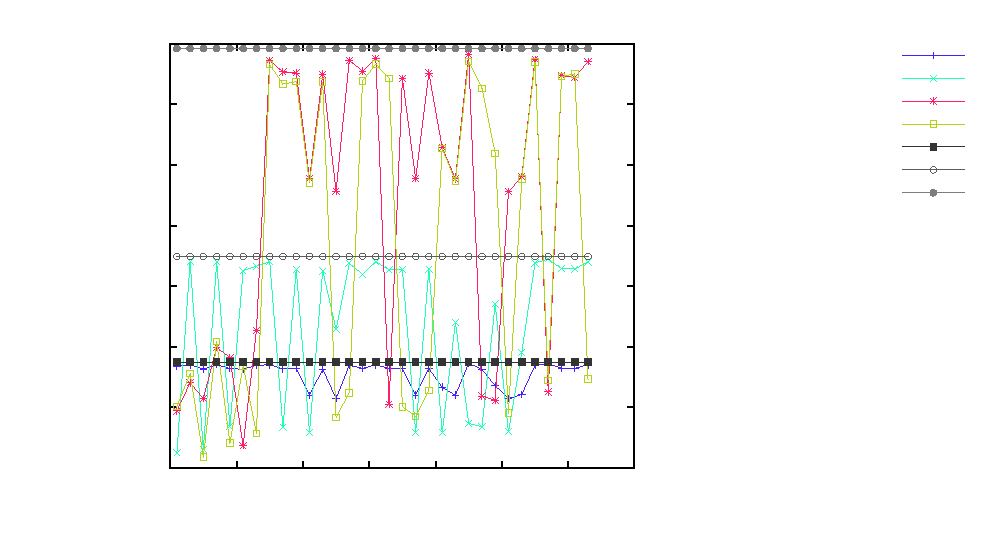
\includegraphics{graph1}}%
    \gplfronttext
  \end{picture}%
\endgroup

	%\caption{Speed of height calculations performed on a subdivided surface} 
	\label{runtimes}
\end{figure}

\begin{table}  [ht]
	\centering
	    \begin{tabular}{lllll}
		padding \verb|#| & 1 thread & 2 threads & 4 threads & 8 threads\\ \hline
			 1 & 336.645 & 50.052 & 188.42 & 203.578\\ 
			 3 & 340.671 & 681.512 & 281.237 & 311.9\\ 
			 5 & 325.773 & 60.015 & 229.057 & 35.603\\ 
			 7 & 341.345 & 679.65 & 398.798 & 417.384\\ 
			 9 & 328.013 & 136.746 & 364.229 & 81.708\\ 
			11 & 325.928 & 651.105 & 73.53 & 337.075\\ 
			13 & 339.033 & 665.709 & 454.8 & 113.712\\ 
			15 & 340.628 & 681.347 & 1344.519 & 1331.212\\ 
			17 & 326.951 & 134.005 & 1307.239 & 1267.278\\ 
			19 & 328.484 & 655.423 & 1303.629 & 1275.71\\ 
			21 & 239.837 & 117.827 & 954.894 & 940.978\\ 
			23 & 326.057 & 650.68 & 1299.702 & 1273.06\\ 
			25 & 229.234 & 457.623 & 913.268 & 167.211\\ 
			27 & 338.9 & 676.013 & 1345.728 & 248.123\\ 
			29 & 328.93 & 639.918 & 1310.198 & 1276.758\\ 
			31 & 340.363 & 680.837 & 1351.127 & 1333.053\\ 
			33 & 329.059 & 654.269 & 210.283 & 1286.229\\ 
			35 & 328.183 & 655.643 & 1286.239 & 202.212\\ 
			37 & 240.275 & 118.158 & 955.255 & 170.186\\ 
			39 & 328.201 & 655.942 & 1303.457 & 255.908\\ 
		    \end{tabular}
	\end{table}

	\end{document}
